\documentclass[letterpaper]{article}
\usepackage{listings}
\usepackage{booktabs}
\usepackage{array}
\usepackage{multirow}
\usepackage{amsmath,amssymb}
\usepackage{hhline}
\usepackage{authblk}
\usepackage[T1]{fontenc}
\usepackage{lipsum}
\usepackage{float}  
\usepackage{graphicx}
\usepackage[export]{adjustbox}
\usepackage{caption}
\usepackage{subcaption}
\usepackage[final]{pdfpages}
\usepackage{wrapfig}
\renewcommand{\baselinestretch}{2}

\usepackage[letterpaper, margin=1in]{geometry}

\begin{document}

\title{MBO and Scheduler User Manual}
\author{Written by: Zach Scheider}
\date{}

\maketitle


\section{MBO and Scheduler}

\subsection{Start Screen}

\begin{figure}[h!]
	\center
	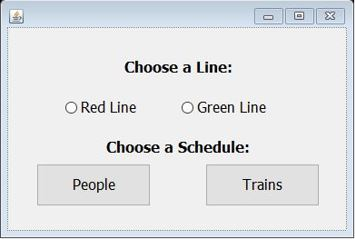
\includegraphics[width=8cm]{main_screen}
	\caption{Start Screen for the MBO and Scheduler.}
\end{figure}


	\subsubsection{Choose a Line}
		\begin{itemize}
			\item Line Selection Radio-buttons - Clicking on the appropriate radio-button will select which line will be used.
		\end{itemize}
	\subsubsection{Choose a Schedule}
		\begin{itemize}
			\item Click on a button to decide whether you want to view the drivers' or trains' schedule for the line that you selected before.
		\end{itemize}
	
\subsection{Schedule Views}

\begin{figure}[h!]
	\center
	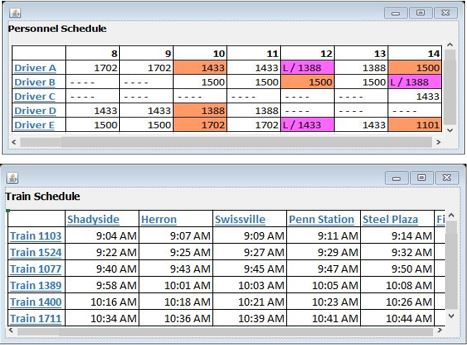
\includegraphics[width=16cm]{schedule_views}
	\caption{Views of the drivers' and trains' schedules.}
\end{figure}

	\subsubsection{Personnel Schedule}
		\paragraph{Row Headings}
			\begin{itemize}
				\item This will display the drivers' names. Clicking on one will display more information about that particular driver.
			\end{itemize}
		\paragraph{Column Headings}
			\begin{itemize}
				\item The time is displayed in the column headings.
			\end{itemize}
		\paragraph{Table Data}
			\begin{itemize}
				\item Inside each cell is the train the driver is operating.
				\item The cells are color coded to display more information.
				\begin{itemize}
					\item Orange means that the driver is scheduled for a break during that time block.
					\item Purple means that the driver is scheduled to take their lunch during that time block.
				\end{itemize}
			\end{itemize}
			
	\subsubsection{Train Schedule}
		\paragraph{Row Headings}
			\begin{itemize}
				\item This will display the trains' IDs. Clicking on one will display more information about that particular train.
			\end{itemize}
		\paragraph{Column Headings}
			\begin{itemize}
				\item This will display the Stations' names. Clicking on one will display more information about that particular station.
			\end{itemize}
		\paragraph{Table Data}
			\begin{itemize}
				\item Inside each cell is the time that the train will arrive at the station.
			\end{itemize}

\subsection{Driver View}

\begin{figure}[h!]
	\center
	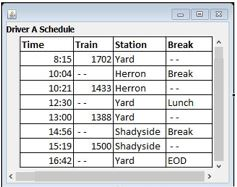
\includegraphics[width=7cm]{driver_view}
	\caption{Views of a particular driver's schedule.}
\end{figure}

	\paragraph{Column Headings}
		\begin{itemize}
			\item The time, train ID, station, and break status are displayed in the column headings.
		\end{itemize}
		
	\subsubsection{Time}
		\begin{itemize}
			\item Inside each cell is the time that the driver will arrive at the station.
		\end{itemize}
	
	\subsubsection{Train}
		\begin{itemize}
			\item Inside each cell is the train that the driver will be operating.
		\end{itemize}
		
	\subsubsection{Station}
		\begin{itemize}
			\item Inside each cell is the station that the driver will arrive at.
		\end{itemize}
		
	\subsubsection{Break}
		\begin{itemize}
			\item Inside each cell is the break status of driver during that block.
		\end{itemize}


\subsection{Station View}

\begin{figure}[h!]
	\center
	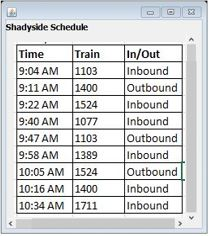
\includegraphics[width=7cm]{station_view}
	\caption{Views of a particular station's schedule.}
\end{figure}

	\paragraph{Column Headings}
		\begin{itemize}
			\item The time, train ID, Inbound/Outbound status are displayed in the column headings.
		\end{itemize}
	
	\subsubsection{Time}
		\begin{itemize}
			\item Inside each cell is the time that a train will arrive at the station.
		\end{itemize}
	
	\subsubsection{Train}
		\begin{itemize}
			\item Inside each cell is the train that will arrive at the station.
		\end{itemize}
	
	\subsubsection{Inbound/Outbound}
		\begin{itemize}
			\item These cells tell the user whether the train is Inbound to the station or Outbound from the station.
		\end{itemize}



\end{document}